\documentclass[11pt,a4paper]{article}

\usepackage[utf8]{inputenc}
\usepackage[a4paper,margin=2.5cm]{geometry}
\usepackage{microtype}
\usepackage{graphicx}
\usepackage{booktabs}
\usepackage{amsmath}
\usepackage{natbib}
\usepackage{hyperref}

\hypersetup{
  colorlinks=true,
  linkcolor=black,
  citecolor=black,
  urlcolor=blue
}

\begin{document}

\begin{titlepage}
  \pagenumbering{gobble}
  \centering
  \vspace*{1.5cm}
  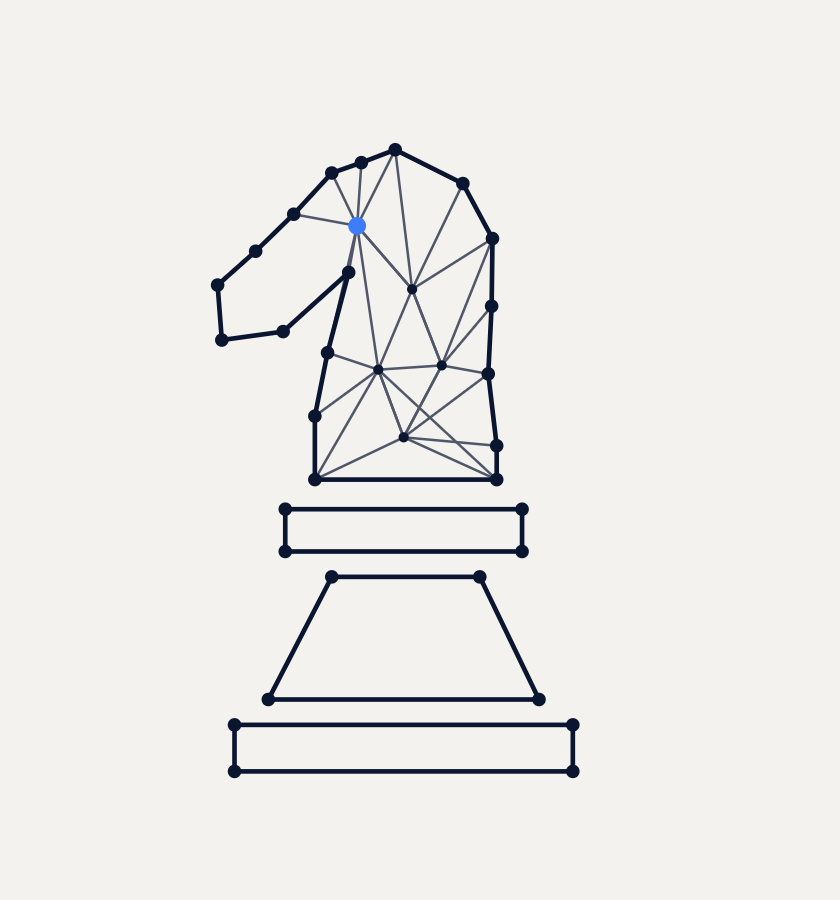
\includegraphics[width=0.28\textwidth]{figures/01 _ Wire mesh (2).png}

  \vspace{1.5cm}
  {\LARGE\bfseries Network Analysis of Chess Opening Transitions\par}

  \vspace{1cm}
  {\large
  Béla Bernasconi\\
  Andrés Santiago Martínez Hernández\\
  Sébastien Pierret\\
  Ali Abdel Ghaffar\par}

  \vfill
  {\large \today\par}
\end{titlepage}
\pagenumbering{arabic}

\begin{abstract}
This report studies chess opening positions as a directed weighted graph built from rated Lichess games.
Nodes represent board states, edges represent observed transitions between states, and edge weights summarize how frequently players choose each continuation.
The goal is to combine graph analysis, custom path scoring, and engine comparison to identify important positions, common transition patterns, position-level outcome tendencies, and human-practical opening paths.
\end{abstract}

\section{Introduction}

Chess games naturally form a sequential decision process: each move transforms one board state into another.
Representing these transitions as a graph makes it possible to study openings using network analysis rather than only move lists or engine evaluations.
This project builds a graph from Lichess PGN data and analyzes how players move through the opening phase.
The central idea is that a position can be valuable not only because an engine evaluates it positively, but also because it is difficult for human opponents to navigate accurately.
For that reason, the analysis combines structural graph measures, empirical game outcomes, and Stockfish comparison.

\section{Data}

The dataset consists of rated standard chess games from the Lichess open database \citep{lichessDatabase}.
Games are filtered before graph construction using player rating and time-control thresholds.
For each retained game, the parser reads the opening sequence up to a fixed depth and records the observed board-state transitions.

\begin{table}[h]
  \centering
  \caption{Dataset and preprocessing parameters. Replace the placeholders with the final values used in the experiment.}
  \label{tab:data-parameters}
  \begin{tabular}{ll}
    \toprule
    Parameter & Value \\
    \midrule
    Source & Lichess rated standard games \\
    Month & 2013-02 / 2015-05 \\
    Minimum Elo & 1000 \\
    Minimum main time & 300 s \\
    Maximum move depth & 20 plies \\
    Position representation & FEN with Zobrist hash key \\
    \bottomrule
  \end{tabular}
\end{table}

\section{Methodology}

\subsection{Graph Construction}

Each unique board position is represented as a node.
For every legal move observed in the filtered games, a directed edge is added from the current position to the next position.
The edge count stores how often that transition appears, and the edge probability is computed from the transition frequency among all outgoing edges of the source position.
The project uses the python-chess library to parse legal moves and to represent board states as FEN strings \citep{pythonChess}.
Each node is keyed by a Zobrist hash and stores its FEN representation, total visit count, and aggregate outcomes.
After loading the raw graph data, nodes are sorted by total visits so that the most common positions can be inspected first.
This ordering is useful for quality control because the initial chess position should be the most visited node.

\subsection{Outcome Value}

Each node stores game outcomes in the order white wins, black wins, and draws.
The expected value of a position is computed as
\begin{equation}
  EV(v) = \frac{W(v) - B(v)}{W(v) + B(v) + D(v)},
\end{equation}
where \(W(v)\), \(B(v)\), and \(D(v)\) are the number of white wins, black wins, and draws observed after visiting position \(v\).
Positive values favor White, negative values favor Black, and values close to zero indicate balanced outcomes.
This normalized value is used as an empirical outcome signal attached to each node.
It does not claim to be a perfect chess evaluation; instead, it measures how games in the dataset tend to end after a given position has occurred.

\subsection{Network Measures}

The report focuses on four network measures implemented with NetworkX \citep{networkx}.
Network density is used as a sanity check for the sparse and sequential nature of the graph.
PageRank identifies transpositional hubs: positions that are important because many relevant paths flow into them.
Betweenness centrality identifies bridge positions or bottlenecks that connect different regions of the opening graph.
Out-degree centrality identifies positions with many continuations, which can be interpreted as positions with high practical branching complexity.

\subsection{Community Detection}

Community detection is used to find groups of closely related game states.
The notebook proposes greedy modularity maximization as the main clustering method because it is suitable for identifying dense local regions in a large graph.
In this setting, communities can be interpreted as opening families or clusters of positions that players tend to reach through similar transition patterns.

\subsection{Depth-Limited Path Scoring}

The custom path analysis is based on a modified depth-limited depth first search.
The algorithm recursively explores continuations from a selected start node until a maximum depth is reached or no successors remain.
At each step, the score contribution for a candidate child node combines the empirical probability of choosing the edge and the expected value of the child position.

\begin{enumerate}
  \item Select a start node \(v\).
  \item Stop if the current search depth equals the depth limit or if \(v\) has no successors.
  \item For each successor \(u\), read the edge probability \(P(v,u)\) and the expected value \(EV(u)\).
  \item Compute a local score contribution \(P(v,u) \cdot EV(u)\).
  \item Continue recursively from \(u\), accumulating the path score.
\end{enumerate}

This creates an outcome-weighted path score that favors lines which are both common enough to be practically relevant and empirically favorable in the dataset.
The method is intentionally different from a pure engine search: it evaluates paths through the lens of human game outcomes and observed transition frequencies.

\subsection{Regression Model}

The notebook also proposes a regression model as a faster approximation of the path-scoring procedure.
The motivation is that exhaustive depth-limited search can become computationally expensive as the graph grows.
A random forest regressor can be trained with scikit-learn on sampled paths represented by features such as path length, average edge probability, minimum edge probability, average expected value, terminal-node expected value, and average out-degree \citep{scikitLearn}.
The target is the heuristic path score produced by the custom algorithm.
If the model performs well, it can quickly estimate promising paths without repeatedly exploring the full search space.

\subsection{Ablation Study}

To assess the custom algorithm, the notebook proposes comparing it against standard graph traversal and shortest-path baselines.
The planned comparison includes the custom DFS, NetworkX DFS, NetworkX BFS, and Dijkstra's algorithm over different dataset subsets.
The evaluation should compare both the resulting path scores and the runtime required to reach similar-quality paths.

\subsection{Stockfish Comparison}

Stockfish is used as an external reference point for selected paths \citep{stockfish}.
The comparison is not treated as a perfect ground truth because the project objective differs from engine optimization.
Stockfish searches for objectively best moves under ideal play, while this project studies paths that perform well in human games.
This distinction is important because many objectively equal positions are easier for one side to play in practice.
Even when an engine evaluates a line as approximately balanced, human players may repeatedly make mistakes if one side has fewer natural or accurate continuations.

The notebook proposes comparing algorithmic path scores with Stockfish evaluations using rank-based agreement, such as Spearman correlation, and top-heavy ranking metrics such as NDCG.
This helps test whether the highest-ranked paths from the graph algorithm align with engine evaluations while still allowing for human-practical divergence.

\section{Results}

This section should report the final graph size, the most visited positions, the strongest transition patterns, the positions with the highest and lowest expected values, and the top-ranked paths from the custom scoring algorithm.

\begin{table}[h]
  \centering
  \caption{Summary statistics for the constructed graph.}
  \label{tab:graph-summary}
  \begin{tabular}{lr}
    \toprule
    Metric & Value \\
    \midrule
    Nodes & TODO \\
    Edges & TODO \\
    Games scanned & TODO \\
    Games retained & TODO \\
    Maximum analyzed depth & TODO \\
    \bottomrule
  \end{tabular}
\end{table}

\begin{figure}[h]
  \centering
  \IfFileExists{figures/example-graph.pdf}{
    \includegraphics[width=0.85\linewidth]{figures/example-graph.pdf}
  }{
    \fbox{\parbox[c][5cm][c]{0.8\linewidth}{\centering Export a graph figure to \texttt{reports/figures/example-graph.pdf}.}}
  }
  \caption{Example graph visualization. Replace this placeholder with an exported figure from the analysis notebook or script.}
  \label{fig:example-graph}
\end{figure}

\subsection{Network Exploration}

The network exploration should summarize density, PageRank, betweenness centrality, and out-degree centrality.
The key interpretation to test is whether popular openings also correspond to favorable expected values, or whether some high-traffic positions mainly reflect player habit.
The PageRank results should highlight unavoidable transpositional hubs, while betweenness should identify positions that act as bridges between opening regions.

\subsection{Path Analysis}

The top paths found by the modified DFS should be reported with their cumulative score, transition probabilities, terminal expected value, and representative board positions.
The notebook notes that visualizing the top paths with color and size can make divergences visible: several strong paths may begin from similar positions and then split at high-branching decision points.
Those divergence points are good candidates for qualitative chess interpretation.

\subsection{Regression Results}

If the random forest experiment is included, report the regression score, feature importances, and examples where the model agrees or disagrees with the custom DFS.
This result should be framed as a computational shortcut rather than a replacement for the graph analysis.

\subsection{Engine Agreement}

The Stockfish comparison should report how closely the graph-based path ranking agrees with engine evaluation.
Spearman correlation can show whether the two methods rank paths similarly overall, while NDCG can emphasize agreement among the top-ranked paths.
Paths with strong graph scores but neutral engine evaluations are especially interesting because they may reveal practical traps or positions that are difficult for humans despite being objectively playable.

\section{Discussion}

Discuss what the network structure reveals about opening behavior.
For example, compare highly visited positions against positions with strong expected values, and describe whether popular choices are also successful choices.
Also note limitations: filtered games may reflect player habits rather than objective chess strength, and early positions are heavily influenced by transpositions.
The Stockfish comparison should also be interpreted carefully.
Engine evaluation measures objective position quality, whereas the graph method measures what happened in the sampled population of games.
Disagreement between the two is not necessarily a failure: it can identify positions where the human decision process differs from engine-perfect play.

\section{Conclusion}

The graph representation provides a compact way to combine move popularity, position outcomes, and structural properties of chess openings.
The modified DFS extends this representation into a path-ranking method that combines transition probability and empirical expected value.
Regression and Stockfish comparison provide two complementary checks: one for computational approximation and one for chess-engine agreement.
The final report should connect these quantitative findings to a clear narrative about how players navigate common opening positions and where practical human difficulty appears in the graph.

\bibliographystyle{apalike}
\bibliography{references}

\end{document}
